\chapter[Hibrid szimulációs program alkalmazása]{Hibrid szimulációs program alkalmazása szeizmikus szigeteléssel ellátott szerkezeten}\label{chap: hibrid alk}

\section {Szeizmikus szigetelés}

{\ }

A földrengésekből adódó károsodások kockázatának csökkentésére különféle technológiák léteznek. A hagyományos megerősítési módok mellett megjelentek a  rezgést csökkentő és elszigetelő szerkezeti rendszerek. Az aktív kontroll rendszereknél (Active Control System - ACS) olyan számítógép vezérlésű lengés-kiegyensúlyozó szerkezetet építenek be, ami külső energia  hatására végez munkát (pl. változtatják a szerkezet merevségét a lökésekkel összhangban). A passzív kontroll rendszerek (Passive Control Systems - PCS) esetében  olyan szerkezetek beépítése történik, amelyek hatással vannak az építmény rezgés-jellemzőire. Léteznek hibrid kontroll rendszerek is ( Hybrid Control Systems - HCS), ahol ACS és PCS rendszereket kombinálnak. Szél és kisebb földrengések esetén PCS rendszerként, nagyobb amplitúdójú dinamikus terhelésnél pedig az ACS rendszerként viselkednek. 

A leggyakrabban használt rendszerek ezek közül a passzív kontroll rendszerek. Ha az építménybe PCS rendszert építenek be elérhető, hogy a  szerkezet és a földrengés periódusa elkülönüljön, így elkerülhető a rezonancia jelensége. A PCS rendszerek két osztályba sorolhatók: szeizmikus szigetelők (Base Isolators) és lengéscsillapítók (Energy Dampers). Ezek közül a továbbiakban a szeizmikus szigetelést mutatom be. 

A szeizmikus szigetelések beépítése viszonylag új technológia. Az első elméletek körülbelül száz éve jelentek meg, azonban  csak a '70-es évek óta  kutatják. Bár csak néhány évtizede vált kivitelezhetővé, mégis rendkívül  elterjedt az alkalmazása.

 A szeizmikus szigetelő rendszerek különösen nagy  jelentősséggel bírnak a már meglévő szerkezetek megerősítésénél, mivel ezeknél a bizonytalan anyagjellemzők és merevségi viszonyok körülményessé  teszik a hagyományos megerősítési módok alkalmazását. Ezekben az esetekben a szeizmikus szigetelés utólagos beépítése megoldást jelent a problémára.
 
 A már meglévő épületek szeizmikus teher elleni megerősítésére több esetben is szükség lehet:
 \begin{itemize}
 \item a kiemelt jelentősségű épületeknél, mint kórházak, mentőállomások, telefonközpontok
 \item műemlék jellegű épületeknél
 \item hidaknál
 \item nagy kihasználtságú épületek, irodaházak, szállodák esetében
 \item veszélyes ipari létesítményeknél, beleértve a víz- és benzintartályokat, atomreaktorokat
 \end{itemize}
 


Szeizmikus szigetelések beépítésénél \cite{simon vigh}  célunk nem a kritikus elemek teherbírásának növelése, hanem a szerkezet válaszának módosításával, energiaelnyeléssel, csillapítással, az igénybevételek és az épületre jutó szeizmikus hatások csökkentése .  
A szeizmikus szigetelőket az alépítmény és a felépítmény közé építik be, mereven rögzítve. Vízszintes merevségük kicsi, ezért a domináns  szeizmikus erők hatása a szerkezetre jelentősen csökken. Az energiát súrlódás vagy hiszterézis viselkedés útján nyelik el. A \ref{fig:szig} ábrán a szeizmikus szigetelés alapelve látható.

\begin{figure}[h!]
\centering
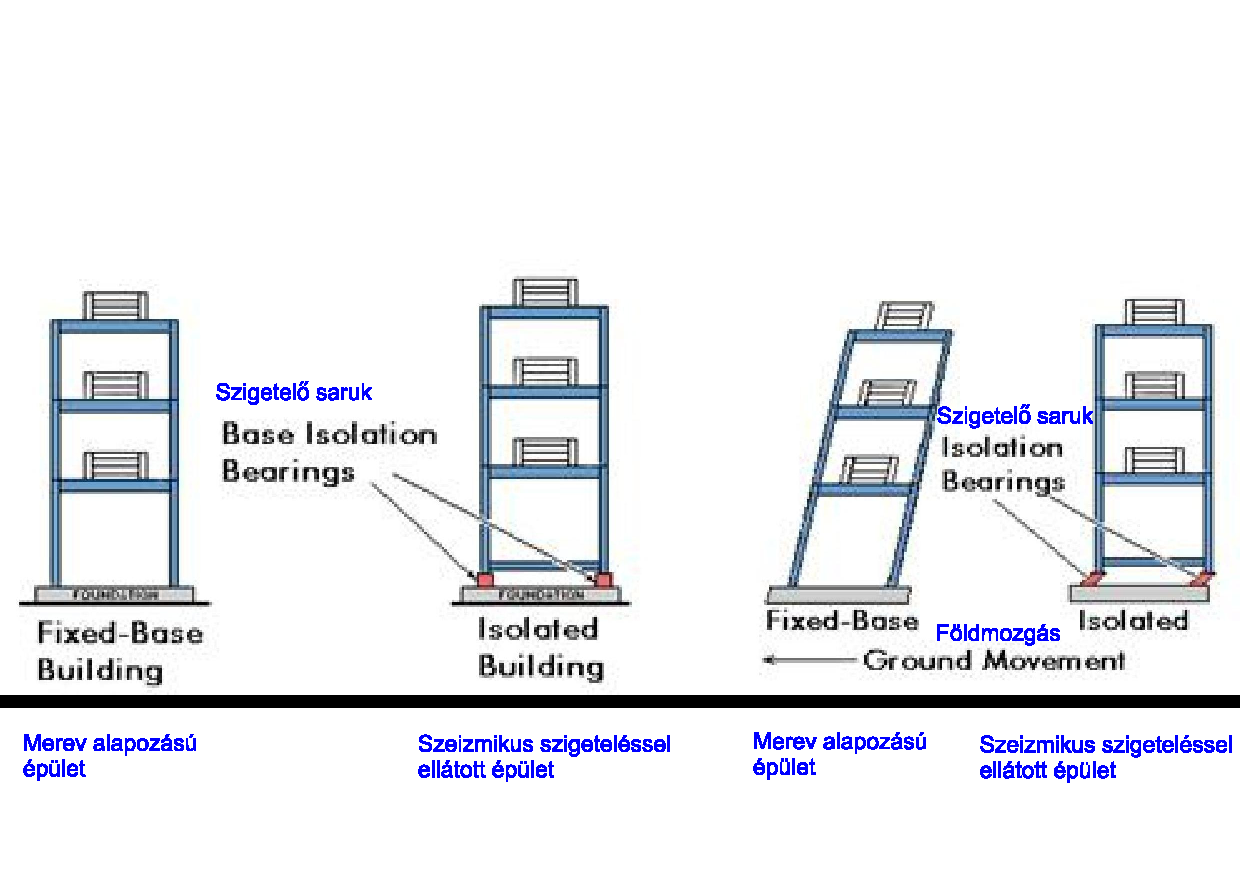
\includegraphics[trim = 0mm 15mm 0mm 25mm, clip, width=0.8\textwidth]{base_isolation.pdf}
\caption{A szeizmikus szigetelés alapelve \cite{hibrid wiki}.}
\label{fig:szig}
\end{figure}

 

Az EN 15129 \cite{antiizé} szerint a szeizmikus szigetelőket  a következőképpen csoportosíthatjuk:
\begin{itemize}
\item elasztomer saru
\item ólom- vagy acélmagos gumi saru
\item egyenes felszínű csúszó saru
\item görbe felszínű csúszó saru
\end{itemize}

Az elasztomer szigetelő saruk természetes vagy  szintetikus gumiból készülnek hengerelt  acéllemezekkel erősítve. Általában rugalmas viselkedésűek. A külső behatásokkal szemben, mint az UV sugárzás, a szerkezet védelméről gondoskodni kell. A berendezések csillapítási mértéke 6-20\% között mozoghat. 
 
A merevítő maggal ellátott gumi saru (Lead Rubber  Bearing -  LRB) az egyszerű elasztomer sarutól annyiban különbözik, hogy a saru belsejében egy acél- vagy ólommag kerül elhelyezésre. Az elhelyezett mag nagyobb vízszintes terhek felvételére képes, így a saru vízszintes irányban merevebbé válik, hiszterézis viselkedése viszont jóval kedvezőbb lesz. A csillapítási mértéke elérheti akár a  40\%-ot is.
 
A csúszólapos saruknál az energiaelnyelés súrlódással történik. A  maximális csillapítási mérték 5-35\% között mozog. Kialakítás szempontjából két fajtájuk van. A  lapos csúszófelülettel kialakított saruk (sliding isolators) hátránya, hogy képtelenek újraközpontosítani (recentering) önmagukat és a felépítményt a terhelés után, erre külön rugalmas elemeket kell beépíteni. A görbe felületű csúszólapos sarunál ezzel ellentétben a konkáv felületnek köszönhetően a vízszintes mozgás  függőlegessel jár együtt. Ezért terhelés közben  a potenciális energia megnő, ami arra készteti a sarut, hogy visszatérjen eredeti, kisebb potenciállal rendelkező helyzetébe. 
  
 
\begin{figure}[h!]
\centering
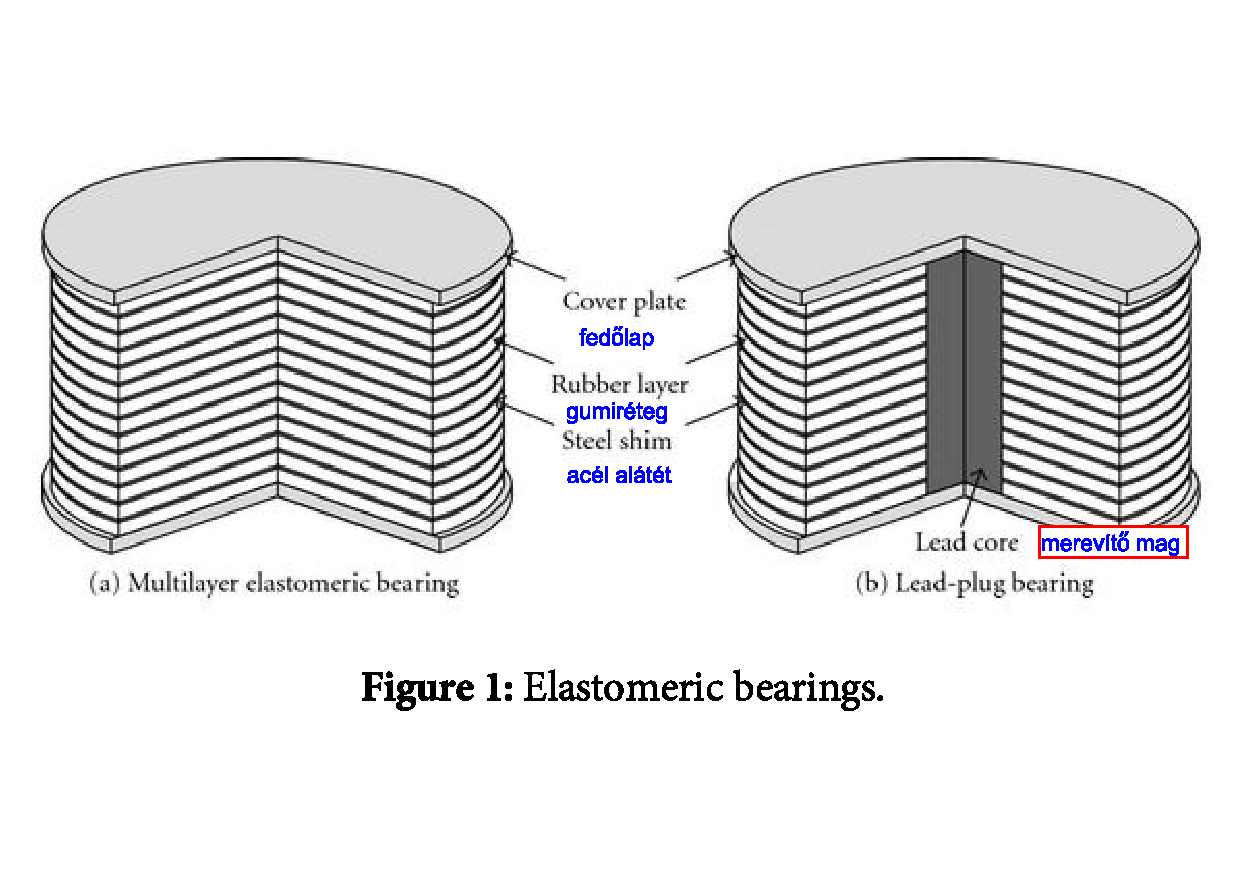
\includegraphics[trim = 0mm 53mm 0mm 15mm, clip, width=0.85\textwidth]{Assessment.pdf}
\caption{Egyszerű és merevítő maggal ellátott elasztomer saru \cite{rubber}.}
\label{fig:linprog}
\end{figure}
 
A szeizmikus szigeteléssel utólag ellátott épületek között az első a Salt Lake City-ben található Város- és Megyeháza volt. A munkálatokat 1989-ben végezték, egyszerű és merevített elasztomer sarukat építettek be. A híres szeizmikus szigeteléssel ellátott épületek között  szerepel a Dél Kaliforniai Egyetem Oktató Kórháza is, amit a merevített gumi szigetelő saruk sikeresen megvédtek az  1994-es Los Angeles-i földrengésben.
 
A következőkben bemutatom a szeizmikus szigetelés csillapító hatását egy konkrét példán keresztül. A szerkezetet összehasonlítom a nem elválasztott szerkezet viselkedésével.
% \url{ http://eda.eme.ro/bitstream/handle/10598/14508/02_FMTU1997%20_%20Gabor%20Aron%20_%20221-224%20old.pdf?sequence=1} }

\section{Szeizmikus szigetelés  csillapító hatásának vizsgálata}

{\ }

A szeizmikus szigetelés csillapító hatását a Chopra könyv \cite{chopra} 23.4.1. pontjában bemutatott ötszintes épületen vizsgáltam  úgy, hogy összehasonlítottam ugyanannak  a szerkezetnek a viselkedését fix megtámasztással és  izoláltan.  A  fix megtámasztású szerkezet elmozdulásait   a \ref{subsec: lin prog szerk} pontban bemutatott  lineáris megoldó programban számítottam,  a szeizmikus szigeteléssel ellátott szerkezetet pedig vizsgáltam a lineáris megoldó programban, illetve a \ref{chap: hibrid progi}. fejezetben ismertetett szimulált hibrid szimulációs programban is. A lineáris megoldó programban  a szigetelés egy lineárisan rugalmas anyagmodellt követ. A hibrid programban egy lineárisan rugalmas - lineárisan felkeményedő képlékeny anyagmodellt alkalmaztam.  A szerkezet többi részét mindhárom esetben lineárisnak feltételeztük. A számításokat ezúttal metrikus rendszerben végeztem.


\begin{figure}%
\centering
\subfigure[][]{%
\label{fig:8rajz-a}%
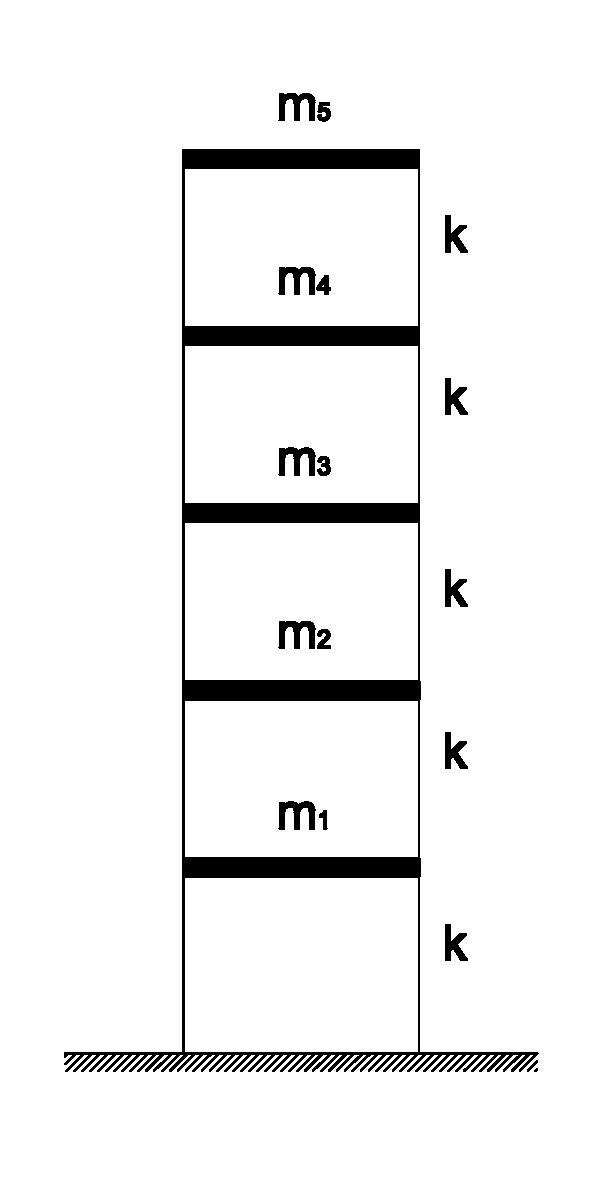
\includegraphics[width=0.3\textwidth]{fix.pdf}}%
\hspace{8pt}%
\subfigure[][]{%
\label{fig:8rajz-b}%
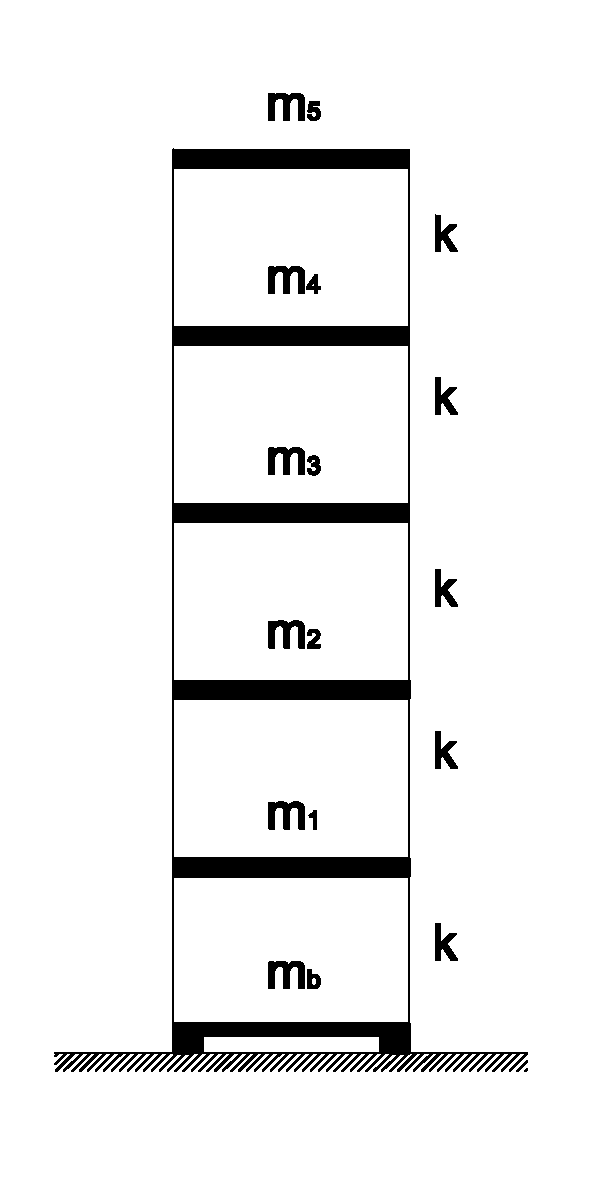
\includegraphics[width=0.3\textwidth]{base.pdf}}%
\caption[A \cite{chopra} 23.4.1 feladatban vizsgált ötszintes keretek.]{A \cite{chopra} 23.4.1 feladatban vizsgált ötszintes keretek: 
\subref{fig:8rajz-a} fix megtámasztású szerkezet;
\subref{fig:8rajz-b} szeizmikus szigeteléssel ellátott szerkezet.}
 \label{fig:8rajz}%
\end{figure}


A szerkezetre mindhárom esetben az El Centro földrengésterhet működtettem. Ennek számítása megegyezik a \ref{subsec:71_hibrid} pontban ismertetettel.


\subsection{Fix megtámasztású szerkezet  lineáris vizsgálata}

{\ }

A fix megtámasztású idealizált szerkezet  a \ref{fig:8rajz-a} ábrán látható. A szerkezetet $\mathbf{M}_{fix}$ tömegmátrix, a $\mathbf{K}_{fix}$ merevségi és $\mathbf{C}_{fix}$ csillapítási mátrixok határozzák meg. Az egyes szintek tömege $m = 100 kips/g = 45,359 t$,  $k$ merevségüket pedig úgy választjuk meg, hogy  a sajátrezgésidő $T_{1,fix} = 0.4 sec$. A szerkezet csillapítását a klasszikus formulával számoljuk, az n-edik szinten $\xi_{fix,n}$ csillapítási tényezővel. A klasszikus csillapítási mátrix $\mathbf{C}_{fix} = \alpha_1\mathbf{K}_{fix}$, $\alpha_1$ értékét $\xi = 2\%$  csillapítási tényezővel számolva.  

A szerkezetet leíró mátrixok számítása:
\begin{align*}
  & \mathbf{M}_{fix}  = m\left[\begin{array}{rrrrr}  1 & 0 & 0 & 0 & 0  \\ 0 & 1 & 0 & 0 & 0 \\ 0 & 0 & 1 & 0 & 0 \\ 0 & 0 & 0 & 1 & 0 \\ 0 & 0 & 0 & 0 & 1  \end{array} \right] t   &  & \mathbf{K}_{fix} = k \left[\begin{array}{rrrrr} 2 & -1 & 0 & 0 & 0  \\ -1 & 2 & -1 & 0 & 0 \\ 0 & -1 &2 & -1 & 0 \\ 0 & 0 & -1 & 2 & -1 \\ 0 & 0 & 0 & -1 & 1 \end{array} \right]\frac{kN}{m}  &  \\
  & \mathbf{C}_{fix}  = \alpha_K\mathbf{K}_{fix}  &  & \alpha_K = \frac{\xi}{\sqrt{\omega_1}} & \\
  & \xi_{fix,n} = \alpha_K\sqrt{\omega_n}& & T_{fix,n} = \frac{2\pi}{\sqrt{\omega_n}} &  
\end{align*} 

\lstinputlisting[firstline=29, lastline=51]{"MATLAB/linear_system_8_fix/init_system.m"}
\lstinputlisting[firstline=74, lastline=89]{"MATLAB/linear_system_8_fix/init_system.m"}

A fix megtámasztású szerkezet első szintjének abszolút (illetve ebben az esetben relatívnak is tekinthető) és tetőponti elmozdulásai a \ref{fig:8_linfix} ábrán láthatók.



\subsection{Szeizmikus szigeteléssel ellátott szerkezet lineáris vizsgálata}

{\ }

A szeizmikus szigeteléssel ellátott épület idealizált modelljét a \ref{fig:8rajz-b} ábra mutatja. A szigetelő szerkezet jellemzésére bevezetjük a következő összefüggéseket:
\begin{subequations}
\label{eq:tb}
\begin{align}
& T_b = \frac{2\pi}{\omega_b}, &  & \omega_b = \sqrt{\frac{k_b}{\mathbf{M}_{fix}+m_b}}; & \\
& \xi_b = \frac{c_b}{2(\mathbf{M}_{fix}+m_b)\omega_b}.&
\end{align}
\end{subequations}

A $T_b$ értéket értelmezhetjük a szigetelő rendszer sajátrezgésidejeként, és $\xi_b$-t a csillapítási tényezőjeként. Ahhoz, hogy a szeizmikus szigetelés hatékonyan csökkentse az épületben a földrengés által kiváltott erőket, $T_b$-nek sokkal hosszabbnak kell lennie, mint $T_{1,fix}$-nek, a merev alátámasztású épület sajátrezgésidejének. Az N emeletes szeizmikus szigeteléssel ellátott szerkezet modellje egy $N+1$ szabadságfokú rendszer nem-klasszikus csillapítással, mivel a szigetelő rendszer csillapítása sokkal nagyobb, mint az épületé.

 Az alaplemez tömege $m_b = m = 45,359 t$ és a szigetelő rendszer merevsége és csillapítása a \eqref{eq:tb} alatti kifejezéseket felhasználva olyan, hogy a sajátrezgésideje $T_b = 2.0 sec$ és a csillapítási tényező $\xi = 10\%$. Az $N+1$ szabadságfokú rendszer tömeg-, merevségi és csillapítási mátrixát rendre $\mathbf{M}$, $\mathbf{K}$ és $\mathbf{C}$ jelöli.


A szerkezetre jellemző mátrixok számítása a fix rendszert leíró mátrixokból:
\begin{align*}
& k_b = \pi^2m6 & & c_b = 0.1m\pi6& \\
& \mathbf{M}_{b}  = \left[\begin{array}{rr}  m & 0 \\ 0 & \mathbf{M}_{fix} \end{array} \right] kg   &  & \mathbf{K}_{b} =  \left[\begin{array}{rr} k_b & -k \\ -k & \mathbf{K}_{fix} \end{array} \right]\frac{kN}{m}  &  \\
& \mathbf{C}_{b}  = \left[\begin{array}{rr} c_b+\mathbf{C}_{fix}(5,5) & -\alpha_Kk \\ -\alpha_Kk & \mathbf{C}_{fix} \end{array} \right] &  \\
  & \xi_{b,n} = \frac{\mathbf{u}_{b,n}^T\mathbf{C}_{b}\mathbf{u}_{b,n}}{\sqrt{\omega_n}}& & T_{b,n} = \frac{2\pi}{\sqrt{\omega_n}} &  
\end{align*}
% & \mathbf{M}_{b}  = m\left[\begin{array}{rrrrrr}  1 & 0 & 0 & 0 & 0 & 0 \\ 0 & 1 & 0 & 0 & 0 & 0 \\ 0 & 0 & 1 & 0 & 0 & 0 \\ 0 & 0 & 0 & 1 & 0 & 0 \\ 0 & 0 & 0 & 0 & 1 & 0 \\ 0 & 0 & 0 & 0 & 0 & 1 \end{array} \right] kg   &  & \mathbf{K}_{b} =  \left[\begin{array}{rrrrrr} k_b & -k & 0 & 0 & 0 & 0 \\ -k & 2k & -k & 0 & 0 & 0 \\ 0 & -k &2k & -k & 0 & 0 \\ 0 & 0 & -k & 2k & -k & 0 \\ 0  & 0 & 0 & -k & 2k -k \\ 0 & 0 & 0 & 0 & -k & k \end{array} \right]\frac{kN}{m}  &  \\

\lstinputlisting[firstline=56, lastline=92]{"MATLAB/hibrid_8/init_system.m"}

A lineárisan számolt szeizmikus szigetelés abszolút, relatív és tetőponti elmozdulásait a \ref{fig:8_linbase} grafikonok mutatják.


\subsection{ Szeizmikus szigeteléssel ellátott szerkezet vizsgálata hibrid szimulációval}

{\ }

A hibrid szimulációban a szerkezet alapadatai és  mátrixai megegyeznek az előbb a szeizmikus szigetelés lineáris vizsgálatánál bemutatottakkal. A lineáris modellhez képest csak a szeizmikus szigetelés anyagában van különbség. A hibrid szimulációs vizsgálat során egy képlékeny anyagot alkalmaztunk a szeizmikus szigetelésnek.

A hibrid programban, konzulensem javaslatára, egy lineárisan rugalmas - lineárisan felkeményedő képlékeny anyagmodellt használtam. Az anyagmodell erő-elmozdulás diagramja a \ref{fig:kepl} ábrán látható. Az  anyag képlékeny állapotban az ábrán jelölt $h$ illetve az $n$ egyenesek mentén változik, attól függően, hogy húzás vagy nyomás áll fenn. Tehermentesítéskor és rugalmas állapotban az ábrán látható $l$ egyenessel párhuzamosan változik. 

\begin{figure}[h!]
\centering
\includegraphics[ width=\textwidth]{kepl_diagramm.pdf}
\caption{A szeizmikus szigetelő elem  képlékeny anyagmodellje a hibrid programban.}
\label{fig:kepl}
\end{figure}

A modell állandó paraméterei a következők:
\begin{description}
\item  [$k_b$]: a kezdeti merevség,
\item  [$k_{pl}$]: aktív képlékeny állapotban a merevség (a kezdeti merevségből számolva: $k_{pl} = \alpha_pk_b$),
\item  [$u_0$]: az első folyáshoz tartozó megnyúlás.
\end{description}
A modell pillanatnyi állapotjellemzője:
\begin{description}
\item  [$u_p$]: az eddig felhalmozott képlékeny alakváltozás (tehermentesítés után a maradó alakváltozás).
\end{description}

A visszatérítő erő számításának lépései időlépésenként:
\begin{enumerate}
\item A felhalmozott alakváltozásból ($u_p$) kiszámoljuk, hogy az $l$ és $h$ illetve $n$ egyenesek hol metszik egymást. A metszéspontokat $u_{h}$ és $u_n$ jelöli.
\begin{align*}
& u_n = -u_0+\frac{1}{1-\alpha_p}u_p & & u_h = u_0+\frac{1}{1-\alpha_p}u_p 
\end{align*}
\item A metszéspontokat ismerve attól függően számítjuk a visszatérítő erőt, hogy az anyag húzott, nyomott, vagy rugalmas illetve passzív képlékeny állapotban van.
\begin{equation*}
f_s = \left\{ \begin{array}{lll} f_s^h, & $ha $  u_h < u & $ (húzott képlékeny állapot)$ \\
								 f_s^l, & $ha $  u_n < u < u_h & $ (rugalmas vagy passzív képlékeny állapot)$ \\ 
								 f_s^n, & $ha $  u < u_n & $ (nyomott képlékeny állapot)$ \end{array}\right.
 \end{equation*}
 
 Ez alapján a visszatérítő erőt az egyes esetekben a következő formulákkal számíthatjuk:
 \begin{align*}
 & f_s^h = k_b((1-\alpha_p)u_0 + \alpha_pu), & \\
 & f_s^l = k_b(u-u_p), & \\
 & f_s^n = k_b((\alpha_p-1)u_0 + \alpha_pu). &
 \end{align*}
\item Ha az anyag aktív képlékeny állapotban van, akkor a képlékeny felhalmozott alakváltozás változik. Új értéke:
\begin{equation*}
u_p = u - \frac{f_s}{k_b}.
\end{equation*}
\end{enumerate}


A hibrid programban az anyagmodell hatása a visszatérítő erő számításánál jelenik meg. Ehhez az  \verb|init_system.m| fájlban definiáltuk a szükséges paramétereket a anyagmodell számításához:
 \lstinputlisting[firstline=134, lastline=142]{"MATLAB/hibrid_8/init_system.m"}
A \verb|resisting_force.m| függvény a következő lesz:
 \lstinputlisting{"MATLAB/hibrid_8/resisting_force.m"}
 
A \ref{fig:hiszt} ábra a szeizmikus szigetelés hibrid programban számolt hiszterézis viselkedését mutatja.
 
\begin{figure}[h!]
\centering
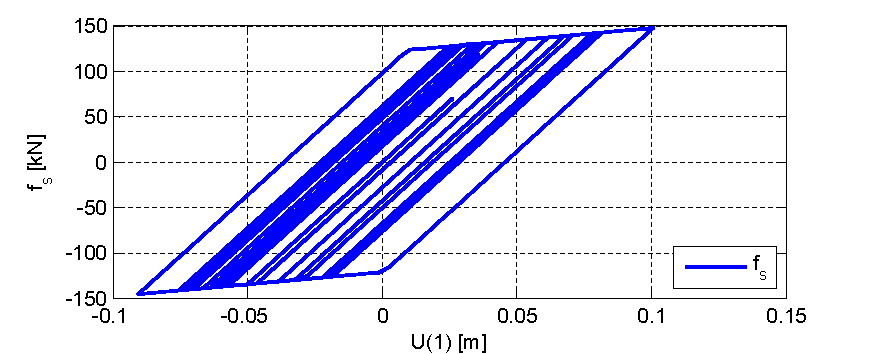
\includegraphics[ width=\textwidth]{83_hiszter.pdf}
\caption{A szeizmikus szigetelő elem  hiszterézis viselkedése a hibrid program számításai alapján.}
\label{fig:hiszt}
\end{figure}

  
A hibrid szimulációs programmal számított képlékeny anyagú szeizmikus szigeteléssel ellátott szerkezet abszolút, relatív és tetőponti elmozdulásait mutatja a \ref{fig:8_hibrid} ábra.





\subsection{Az eredmények összehasonlítása}

{\ }

A következőkben a fix megtámasztású szerkezet, a lineárisan rugalmas és a képlékeny szeizmikus szigeteléssel ellátott szerkezet számítási eredményeit hasonlítjuk össze az abszolút, a relatív és a tetőponti elmozdulások, valamint a keletkező  nyíróerők szerint. Ezeknek az egyes számításokból származó maximális értékeit a \ref{8_table} táblázat foglalja össze.

Az eredményekből kitűnik, hogy a szeizmikusan szigetelt épületek maximális abszolút elmozdulásai képlékeny esetben 5-ször, lineárisan rugalmas esetben több, mint 8-szor nagyobbak, mint a fix megtámasztású szerkezetnél, azonban a relatív elmozdulások esetében ez az arány fordított. A merev megtámasztású épület maximális relatív elmozdulása több, mint négyszerese a képlékeny, és majdnem nyolcszorosa a lineárisan rugalmas szigetelésű szerkezetnél számított relatív elmozdulásoknak. Ebből az következik, hogy  a maximális nyíróerők is ugyanakkora arányban csökkennek szeizmikus szigetelés esetében. A tetőponti elmozdulások fix megtámasztásnál az első szint elmozdulásainak többszörösére adódnak, míg szeizmikus szigetelésnél minimális az eltérés a tetőpont és az első szint maximális elmozdulásai között.

Mindez azt mutatja, hogy szeizmikus szigetelés esetében az épület inkább merevtest-szerűen eltolódik, a nagy deformációkat a szigetelés veszi fel, így a szerkezetben sokkal kisebb igénybevételek keletkeznek. 

\begin{figure}[!ht]%
\centering
\subfigure[][]{%
\label{fig:8_linfix-a}%
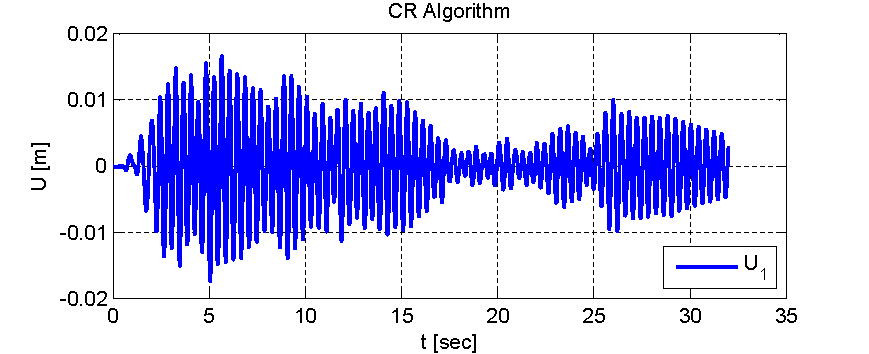
\includegraphics[width=0.9\textwidth]{81_u2.pdf}}%
\\
\subfigure[][]{%
\label{fig:8_linfix-b}%
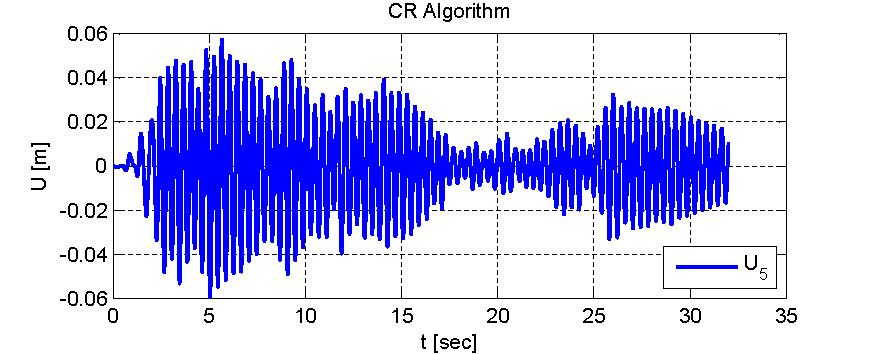
\includegraphics[width=0.9\textwidth]{81_u5.pdf}}%
\caption[A lineáris programban vizsgált merev alapú  szerkezet elmozdulásai.]{A lineáris programban vizsgált merev alapú  szerkezet elmozdulásai:
\subref{fig:8_linfix-a} az első szint abszolút elmozdulásai; 
\subref{fig:8_linfix-b} tetőponti elmozdulások.}%
\label{fig:8_linfix}%
\end{figure}

\begin{figure}[!ht]%
\centering
\subfigure[][]{%
\label{fig:8_linbase-a}%
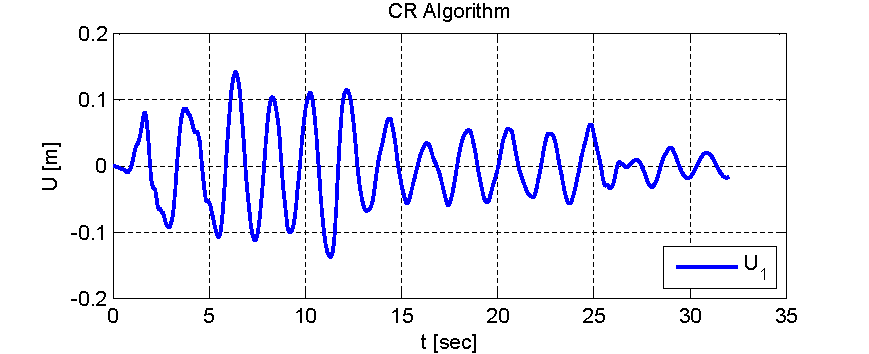
\includegraphics[width=0.9\textwidth]{82_u2.pdf}}%
\\
\subfigure[][]{%
\label{fig:8_linbase-b}%
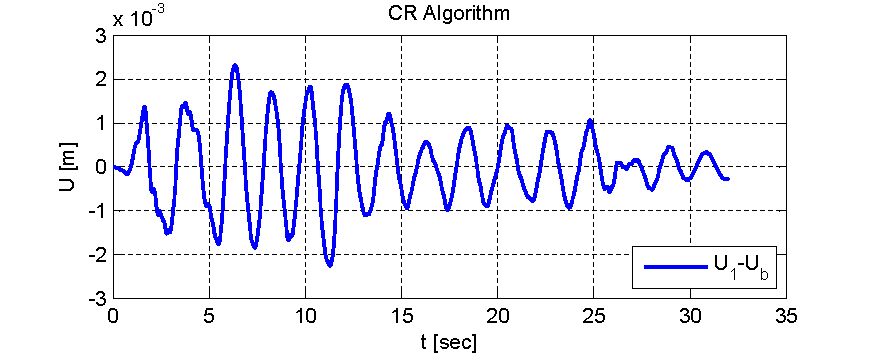
\includegraphics[width=0.9\textwidth]{82_u_rel.pdf}}%
\\
\subfigure[][]{%
\label{fig:8_linbase-c}%
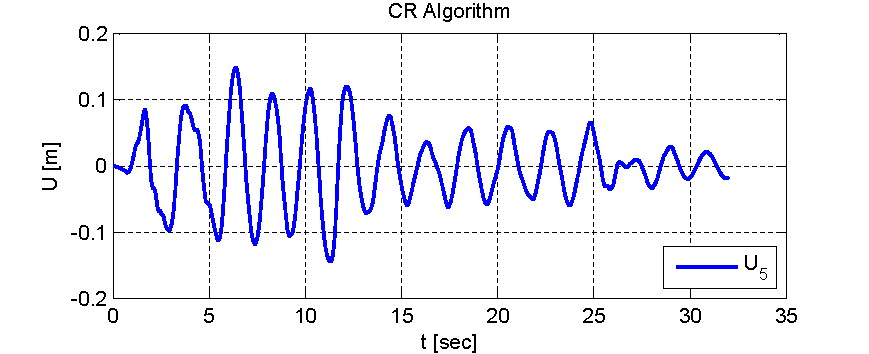
\includegraphics[width=0.9\textwidth]{82_u5.pdf}}%
\caption[A lineáris programban vizsgált szeizmikus szigeteléssel ellátott szerkezet elmozdulásai.]{A lineáris programban vizsgált szeizmikus szigeteléssel ellátott szerkezet elmozdulásai:
\subref{fig:8_linbase-a} az első szint abszolút elmozdulásai;
\subref{fig:8_linbase-b} az első szint relatív elmozdulásai; 
\subref{fig:8_linbase-c} tetőponti elmozdulások.}%
\label{fig:8_linbase}%
\end{figure}



\begin{figure}[!ht]%
\centering
\subfigure[][]{%
\label{fig:8_hibrid-a}%
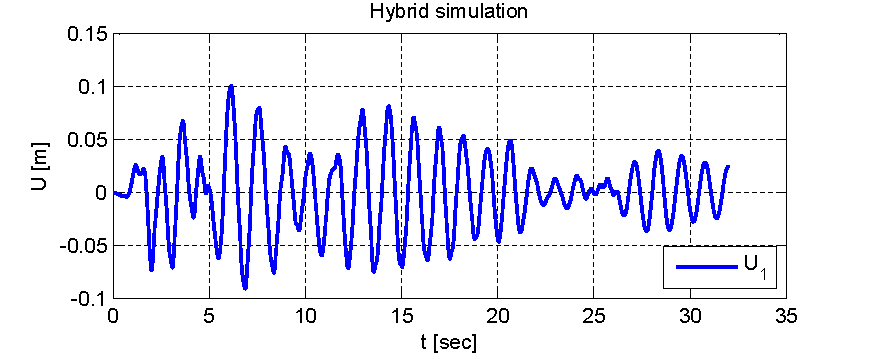
\includegraphics[width=0.9\textwidth]{83_u2.pdf}}%
\\
\subfigure[][]{%
\label{fig:8_hibrid-b}%
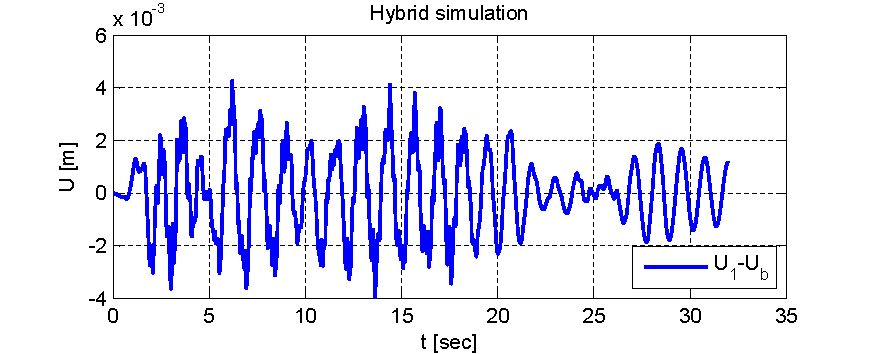
\includegraphics[width=0.9\textwidth]{83_u_rel.pdf}}%
\\
\subfigure[][]{%
\label{fig:8_hibrid-c}%
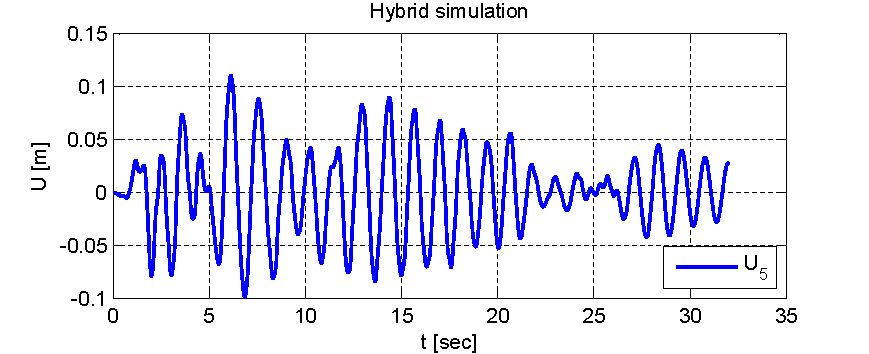
\includegraphics[width=0.9\textwidth]{83_u5.pdf}}%
\caption[A hibrid programban vizsgált szeizmikus szigeteléssel ellátott szerkezet elmozdulásai.]{A hibrid programban vizsgált szeizmikus szigeteléssel ellátott szerkezet elmozdulásai:
\subref{fig:8_hibrid-a} az első szint abszolút elmozdulásai;
\subref{fig:8_hibrid-b} az első szint relatív elmozdulásai; 
\subref{fig:8_hibrid-c} tetőponti elmozdulások.}%
\label{fig:8_hibrid}%
\end{figure}



\begin{table}[h!]
\centering
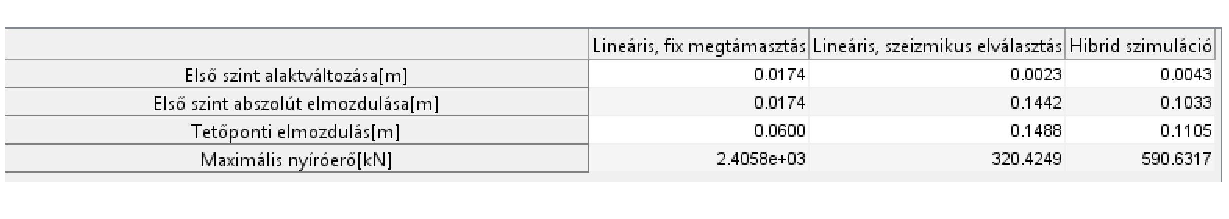
\includegraphics[trim = 20mm 0mm 0mm 0mm, clip, width=\textwidth]{8_table.pdf}
\caption{A fix megtámasztású és a szeizmikus szigeteléssel ellátott épület maximális elmozdulásai és nyíróerői.}
\label{8_table}
\end{table}

Elmondható továbbá, hogy a szeizmikus szigetelés elsősorban a szigetelő rendszer  módjának sajátrezgésideje  miatt csökkenti a maximális nyíróerők értékét, mert a legtöbb válasz esetében ez sokkal hosszabb, mint a merev  épület sajátrezgésideje, és ez sokkal kisebb válaszspektrum ordinátához vezet.  A tervezési válaszspektrumot szilárd talajon, merev megtámasztású szerkezet esetében  a válaszspektrum  gyorsulásérzékeny területének lapos részében  a sajátperiódusidővel jellemezhetjük. A magasabb  módokat a földmozgás nem gerjeszti (még ha a pszeudo-gyorsulások nagyok is), mert a modális válaszok nagyon kicsik. 

Az eredményekből arra következtethetünk, hogy a szeizmikus szigetelés hatékonyan csökkenti a földrengés okozta erőket a szerkezetekben. Ennek elsődleges oka az  első mód periódusának meghosszabbodása. A szigetelő rendszer csillapító hatása és a járulékos energia disszipáció csak másodlagos tényező a strukturális válasz csökkentésében. 


